\section{Motivation}
\subsection{Superlight Clients}

Given an honestly adopted chain, consensus security is based on the premise that
it is difficult to create a competing chain which deviates significantly and has
more proof-of-work than the existing honestly adopted chain. To determine which
financial history is the valid one, a \emph{verifier} node booting for the first
time into the network, connects anew to multiple \emph{provers}, at least one of
which is assumed to be honest. The verifier then downloads all available
blockchains from its peers and adopts the longest one. The verifier must choose
the chain that respects the protocol rules and corresponds to the most
proof-of-work. In order to do that, the proof-of-work of every block in the
chain must be presented and verified.

\begin{figure}[tb]%{{{
  \centering
  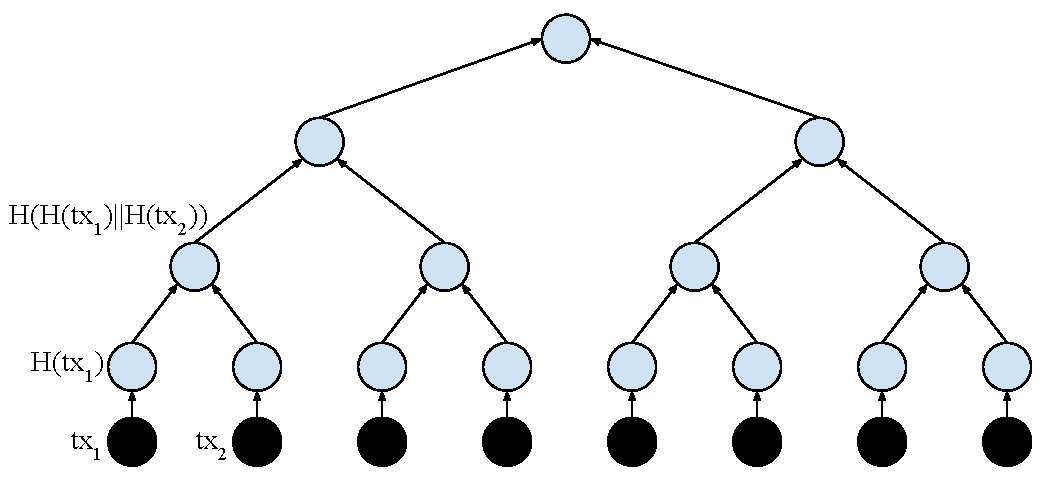
\includegraphics[width=0.9 \textwidth]{chapters/introduction/figures/merkle-tree.pdf}
  \caption{
    A Merkle Tree of transactions making use of a cryptographicallys secure hash
    function $H$. Black nodes indicate raw transactions.
    Lightly shaded nodes indicate hashes. The root is shown at the top.
  }
  \label{fig.merkle}
\end{figure}%}}}

Nodes on the blockchain that maintain the whole history of transactions and
chain are known as \emph{full nodes}. Typically, miners are full nodes, but some
non-mining nodes are also full nodes.
Proof-of-work blockchain clients such as mobile wallets today are based on the
Simplified Payment Verifications (SPV) protocol, which was described in the
original Bitcoin paper~\cite{bitcoin}, and allows them to sychronize with the
network by downloading only block \emph{headers} and not the entire blockchain with
transactions. However, such initial synchronization still requires receiving all
the block headers.

Instead of having each block contain all of its
transactions and performing proof-of-work on it, transactions are first hashed
into a special structure known as a Merkle Tree. A Merkle Tree of a transaction
sequence $\overline{x}$ is structured as illustrated in Figure~\ref{fig.merkle}. Using a cryptographically
secure hash function $H$, each transaction is hashed to obtain its transaction
\emph{id}. Subsequently, each two ids are concatenated together and hashed again
to obtain their parent. These parents are again concatenated and hashed
together to obtain \emph{their} parent, until we arrive at a single \emph{root}
node $x$ which contains a hash representation of every transaction in
$\overline{x}$. The proof-of-work of the block is then computed by finding a
$\textsf{nonce}$ such that $H(x \concat \textsf{nonce} \concat h') \leq T$. The
transactions $\overline{x}$ are known as the \emph{block content}, while the
portion $x \concat \textsf{nonce} \concat h'$ which is hashed for proof-of-work
purposes is known as the \emph{header}.

This chain $\chain$ of block headers grows linearly in time. To put the problem
in perspective and motivate the question, at the time of writing, Ethereum's
blockchain (as measured by the amount of data that needs to be downloaded to
synchronize a full node) is currently more than $250$GB, and the size of block
headers is $4.6$GB. The latter amount is currently too large for a user-friendly
mobile wallet.

The problem we concern ourselves with is whether it is possible to optimize this
protocol, achieving communication $o(|\chain|)$. We study the question of
whether better protocols exist and in particular if downloading fewer block
headers is sufficient to securely synchronize with the rest of the blockchain
network. Our requirement is that the system remains decentralized and that
useful facts about the blockchain (such as the Merkle root of current account
balances in Ethereum) can be deduced from the downloaded data. This means that
we don't want to utilize techniques such as checkpointing (in which the verifier
software is patched by its trusted developer to include a later block as
a \emph{neon genesis} replacement to the genesis block) or trusting a server to
give us the correct blockchain.

Our setting is as follows. A \emph{superlight} verifier wakes up having only the
first block of the blockchain, the genesis block. In the meantime, the
blockchain has grown and contains many blocks. The verifier wishes to know
whether a transaction is confirmed to decide if a payment has been made. It
connects to multiple other \emph{full nodes}, that we term \emph{provers}
throughout this work, who maintain the whole blockchain. At least one connection
will be to an \emph{honest node}. All the provers send some claims to the
verifier, some claiming that the transaction is confirmed, while others that it
is not. The goal of the verifier is to decide which of these claims is true. The
claims are accompanied by \emph{evidence} to illustrate them, but must be short
in length so that the client can synchronize quickly. In particular, we aim for
exponentially shorter messages $\bigO(polylog(|\chain|))$ instead of the
standard $\bigO(|\chain|)$ than an SPV node requires. These superlight nodes are
useful when a client such as a mobile wallet wishes to synchronize with the
network quickly. Other facts beyond transaction inclusion, such as account
balances, are also useful to prove.

The question the verifier is trying to answer is not simply whether the
transaction has been included in \emph{some} valid block, but whether that block
belongs to the longest chain and hence the economic participants will also agree
that the transaction took place. For the proof-of-work case, this chain
corresponds to the chain containing the most proof-of-work that respects the
protocol rules (such as the occasional recalculation of the target $T$ due to
changes in the total mining power of the network). For proof-of-stake, this
chain corresponds to the longest chain which has valid signatures by the
majority of the stakeholders at each point in time, keeping in mind that stake
is shifting from epoch to epoch. In both cases we are trying to create succinct
proofs \emph{about} the fact that proof-of-work or proof-of-stake took place
without presenting every proof-of-work nonce or every proof-of-stake signature.
This gives rise to \emph{Proofs of Proof-of-Work} and stake.

While it is useful for mobile wallets to synchronize quickly, if a good protocol
for superlight nodes is developed, one natural question that arises is whether
the same protocol can also be used for full nodes and miners. This would help
quickly create a new miner and have it working on the chain without needing a
long synchronization time. Can miners, like superlight clients, also synchronize
quickly with the rest of the network while achieving security comperable to a
full node? And if so, do we need any extra assumptions and what are the security
limitations of such a model?

\subsection{Interoperability}
Since the invention of Bitcoin in 2009, numerous other cryptocurrencies have
followed, improving upon Bitcoin on several aspects. The most prolific of these
is \emph{Ethereum}~\cite{buterin}, which introduces the concept of \emph{smart
contracts}. These Turing-complete programs enable developers to define complex
conditions which must be satisfied to spend money, beyond the simple signatures
that Bitcoin allows as conditions for spending. They are programmed in
specialized programming languages such as Solidity and run on top of the
Ethereum Virtual Machine~\cite{wood}. Each contract is a sovereign entity that
can own money and define the rules under which this money can be spent. These
contracts execute autonomously. Their correct execution is verified by miners on
the network, in a similar way that signatures are verified in Bitcoin's case.

Other cryptocurrencies that include significant contributions and
experimentation are \emph{Litecoin}~\cite{litecoin} which aims to be more
egalitarian~\cite{egalitarianism}; \emph{Monero}~\cite{cryptonote} and
\emph{ZCash}~\cite{zerocoin,zcash}, which improve upon the generally
poor~\cite{fistful,quantitative-bitcoin-analysis,tumblebit} privacy of
Bitcoin; \emph{Namecoin}~\cite{namecoin} which was a first attempt at creating a
decentralized DNS alternative; \emph{Dogecoin}~\cite{dogecoin}, which experiments with
inflationary economics in contrast to Bitcoin's deflationary nature;
\emph{Bitcoin Cash}~\cite{btcVSbch}, which experiments with larger block sizes; and
\emph{Cardano}~\cite{ouroboros}, which uses proof-of-stake instead of proof-of-work.

It is possible to \emph{trade} one coin for the other. For example, if one
wishes to exchange Bitcoin for Ethereum, they need to find a counterparty who
wishes to exchange Ethereum for Bitcoin (this is generally easy to do through
centralized services). However, each of these blockchain systems remains
isolated. The concept of a \emph{cryptocurrency} and its respective \emph{chain}
remain intertwined: A Bitcoin lives in the Bitcoin chain, while an Ether lives
in the Ethereum chain. The \emph{interoperability} problem pertains to the
ability to move a cryptocurrency from its native chain to a remote chain,
a one-way peg\index{One-way Peg}, and then back, a two-way
peg\index{Two-way Peg}. If Bitcoin and Ethereum were interoperating, it would be
possible to move one Bitcoin from the Bitcoin chain to the Ethereum chain and
back. The Bitcoin would retain its \emph{nature} during its lifespan within the
Ethereum chain. It would always be a Bitcoin, not an Ether. For example, it
would maintain the same exchange rate against other currencies. While on the
Ethereum chain, it would also enjoy the benefits of the Ethereum ecosystem. For
example, it would make itself subject to smart contracts and enjoy the faster
confirmation speed of Ethereum. At the same time, it would make itself subject
to the security assumptions of Ethereum. For example, it could subject itself to
more limited security protection under a smaller amount of honest computational
power devoted to the mining of the chain it lives on. The bitcoin would have the
benefits and shortcomings of the Ethereum environment only as long as it lives
on the foreign blockchain. When it returns back to its native chain, it should
again behave within the context of the Bitcoin blockchain. The bitcoin has
become \emph{decoupled} from its blockchain. This is illustrated in
Figure~\ref{fig.two-way-peg}.

\begin{figure}[tb]%{{{
  \centering
  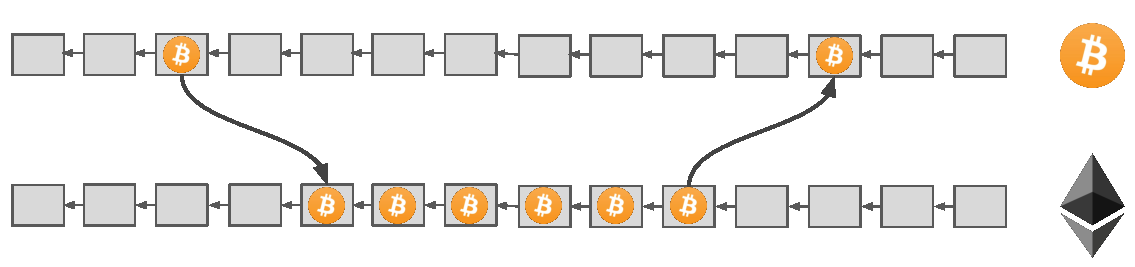
\includegraphics[width=0.9 \textwidth]{chapters/introduction/figures/two-way-peg.pdf}
  \caption{
    A motivating but imaginary two-way peg. A bitcoin is moved from its native
    Bitcoin chain to the Ethereum chain and back. While on the Ethereum chain,
    it is still a bitcoin.
  }
  \label{fig.two-way-peg}
\end{figure}%}}}

More generally, and beyond the transfer of a cryptocurrency asset from one
blockchain to another, it is useful to allow one blockchain to consume
information pertaining to another. Today, smart contracts are confined to access
data only within the blockchain they run on, such as data maintained within the
state of the smart contract itself. Access to external data requires a trusted
third party or group thereof to vouch for the data validity~\cite{towncrier}.
As contracts can represent complex financial conditions and trust relationships,
it is useful to give them the ability to take decisions based on \emph{events}
that take place on different chains. One example could be an Ethereum contract
which gives out shares in a decentralized company (in the form of tokens)
conditioned on the fact that a series of Bitcoin payments have been made in
regular intervals during a predetermined period of time. Another example could
be an insurance contract running on the Ethereum blockchain which, conditioned
on the fact that a particular Bitcoin account fails to receive a predetermined
amount of money until a particular point in time, releases an Ethereum payment
to its policyholder. As one can readily see from these not so complex examples,
such contract conditions that go beyond a simple payment cannot be readily
encoded in the form of an atomic swap or a two-way peg and may not even have a
definite counter-party in each chain.

As such, we are looking for a generic cross-chain communication mechanism which
allows blockchains to interoperate, achieving one-way pegs, two-way pegs, as
well as generic information transfers. Such a system should allow smart
contracts on one blockchain to receive and react to events taking place on
another blockchain without the need of trusted parties. We term this generic
communication mechanism a \emph{sidechain}\footnote{We note here that previous
work has used this term in a narrower context than the generic information
transfer we propose here. This is one reason why the term \emph{cross-chain
communication} for a generic protocol may be preferable.}. Despite their widely
agreed usefulness there exist currently no sidechain constructions that are
decentralised, efficient, and generic at the same time. One critical challenge
in desigining these protocols is that the aim is to allow the two chains to
remain \emph{miner isolated}. This means that, while users could maintain
wallets in multiple chains and observe them for transactions of their interest,
as well as forward information between the chains, the \emph{miners} that
run the consensus protocol in each chain cannot be required to connect to
multiple networks. For example, it is desirable that Ethereum can react to
Bitcoin events without requiring the Ethereum miners to connect to (or even know
about the existence of) the Bitcoin network.

% Sidechains can exist in two forms. In the first case, they are simply a
% mechanism for two existing \textit{stand-alone blockchains} to communicate, in
% which case any of the two blockchains can be the sidechain of the other and they
% are treated as equals. In the second case, the sidechain can be a ``child'' of
% an existing blockchain, the \textit{mainchain}, in that its genesis block, the
% first block of the blockchain, is somehow seeded from the parent blockchain and
% the child blockchain is meant to depend on the parent blockchain, at least
% during an initial bootstrapping stage.

% A sidechain system can choose to enable certain types of interactions between
% the participating block\-chains. The most basic interaction
% is the transfer of assets from
% one blockchain to another. In this application, the nature of the asset
% transferred is retained in that it is not transformed into a different class of
% asset.
% As such, it maintains its value and may also be transferred back.
% The ability to move assets back and
% forth between two chains is sometimes referred to as a \textit{2-way peg}. Provided
% the two chains are both secure as individual blockchains, a secure
% sidechain protocol construction allows this security to be carried on to
% cross-chain transfers.

Interoperability can also be a useful mechanism to enable interfacing between
decentralized blockchains and more traditional centralized systems such as
accounts whose balances are held by custodians and are subject to the traditional
laws of particular countries. Such a construction could allow for a smoother
transition from the legacy monetary system to a blockchain-enabled system. The
same mechanisms that allow a smart contract in Ethereum to verify a remote
Bitcoin payment can be used to allow a \emph{permissioned} chain (in which the
consensus is achieved by majority voting between a centralized committee) to
verify a Bitcoin payment without requiring its consensus maintainers to connect
to the Bitcoin network. It is, of course, trivial to write an Ethereum verifier
that checks whether a transaction has been confirmed within such a permissioned
network (by simply verifying and counting signatures). Therefore in this thesis
we will concentrate on consuming data from decentralized chains, as the other
way around is straightforward.

While sidechains were not originally proposed for scalability purposes, they can
also be used to off-load the load of a blockchain in terms of transactions
processed. For this purpose, a particular blockchain, which we will call the
\emph{main chain}, that wishes to off-load its load can create multiple separate
chains, the \emph{side chains}, that maintain consensus independently. A
cross-chain protocol can then be used to connect each side chain to the main
chain, with the main chain functioning as a financial hub. While communication
protocols between the main chain and the side chain can be symmetric, their use
cases are different. In this application, the use of the main chain is as a
permanent store of value as well as an interface between different side chains,
while each side chain is used for everyday transactions. As long as 2-way pegs
are enabled, a particular sidechain can offer specialization by, e.g., industry,
in order to avoid requiring the mainchain to handle all the transactions
occurring within a particular economic sector. As long as the majority of
transactions does not cross economic sectors, this provides a straightforward
and simple way to ``shard'' blockchains~\cite{sharding,omniledger,rapidchain}.
Another way of sharding could be by geographical location.

Lastly, a child side chain can be created from a parent main chain as a means of
exploring a new feature, e.g., in the scripting language, or the consensus
mechanism without requiring a soft, hard, or velvet fork~\cite{nipopows,velvet}.
The side chain does not need to maintain its own separate currency, as value can
be moved between the sidechain and the main chain at will. If the feature of the
sidechain proves to be popular, the main chain can eventually be abandoned by
moving all assets to the sidechain, which can become the new main chain. In
fact, such experimentation with new features was one of the original motivators
for sidechains~\cite{sidechains}.

Given the benefits listed above, there is a pressing need to address the
question of sidechain security and feasibility, which so far has not received
any formal treatment.
